\section{Experiments}
In this section, we evaluate our proposed algorithm IROC on both synthetic data sets and real data sets and compare it with $4$ relevant algorithms. The code of the comparison methods are obtained from the authors. Experiments have been performed on a workstation with $2.9GHz$ Intel Core $i7$ and $8G$ memory.

\subsection{Synthetic Data sets}
\subsubsection{Data sets}
The sketches of three synthetic data sets are shown in Tab. \ref{tab:syn}. Each circle represents a densely connected cluster and the shadow part denotes the overlapping part in which vertices are assigned to multiple clusters. The synthetic attributed graphs are generated with the following parameters: Each cluster contains $200$ vertices ($n_c = 200$); $n_o$ is the number of vertices in the overlapping part; the density of edges in and between clusters are $0.8$ and $0.1$ respectively ($d_c=0.8, d_b=0.1$). The subspace of attributes of the three synthetic data sets are also shown in Table \ref{tab:syn}. The number of dimensionality of the subspace of each cluster is denoted as $n_d$ and $2$ dimensions are overlapping ($n_{od} = 2$). Each cluster contains nearly same category in its subspace attributes and $r=0.05$ of them are randomly generated with other categories. The categories which do not belong to the subspace are randomly generated. 
\begin{table*}[t]
\centering
\caption{Parameter Settings for Generating Synthetic Data Set}
\begin{tabular}{|c|c|c|c|}
\hline
Datasets & Syn1 & Syn2 & Syn3\\
\hline
\tabincell{c}{Sketch} & \raisebox{-0.9\height}{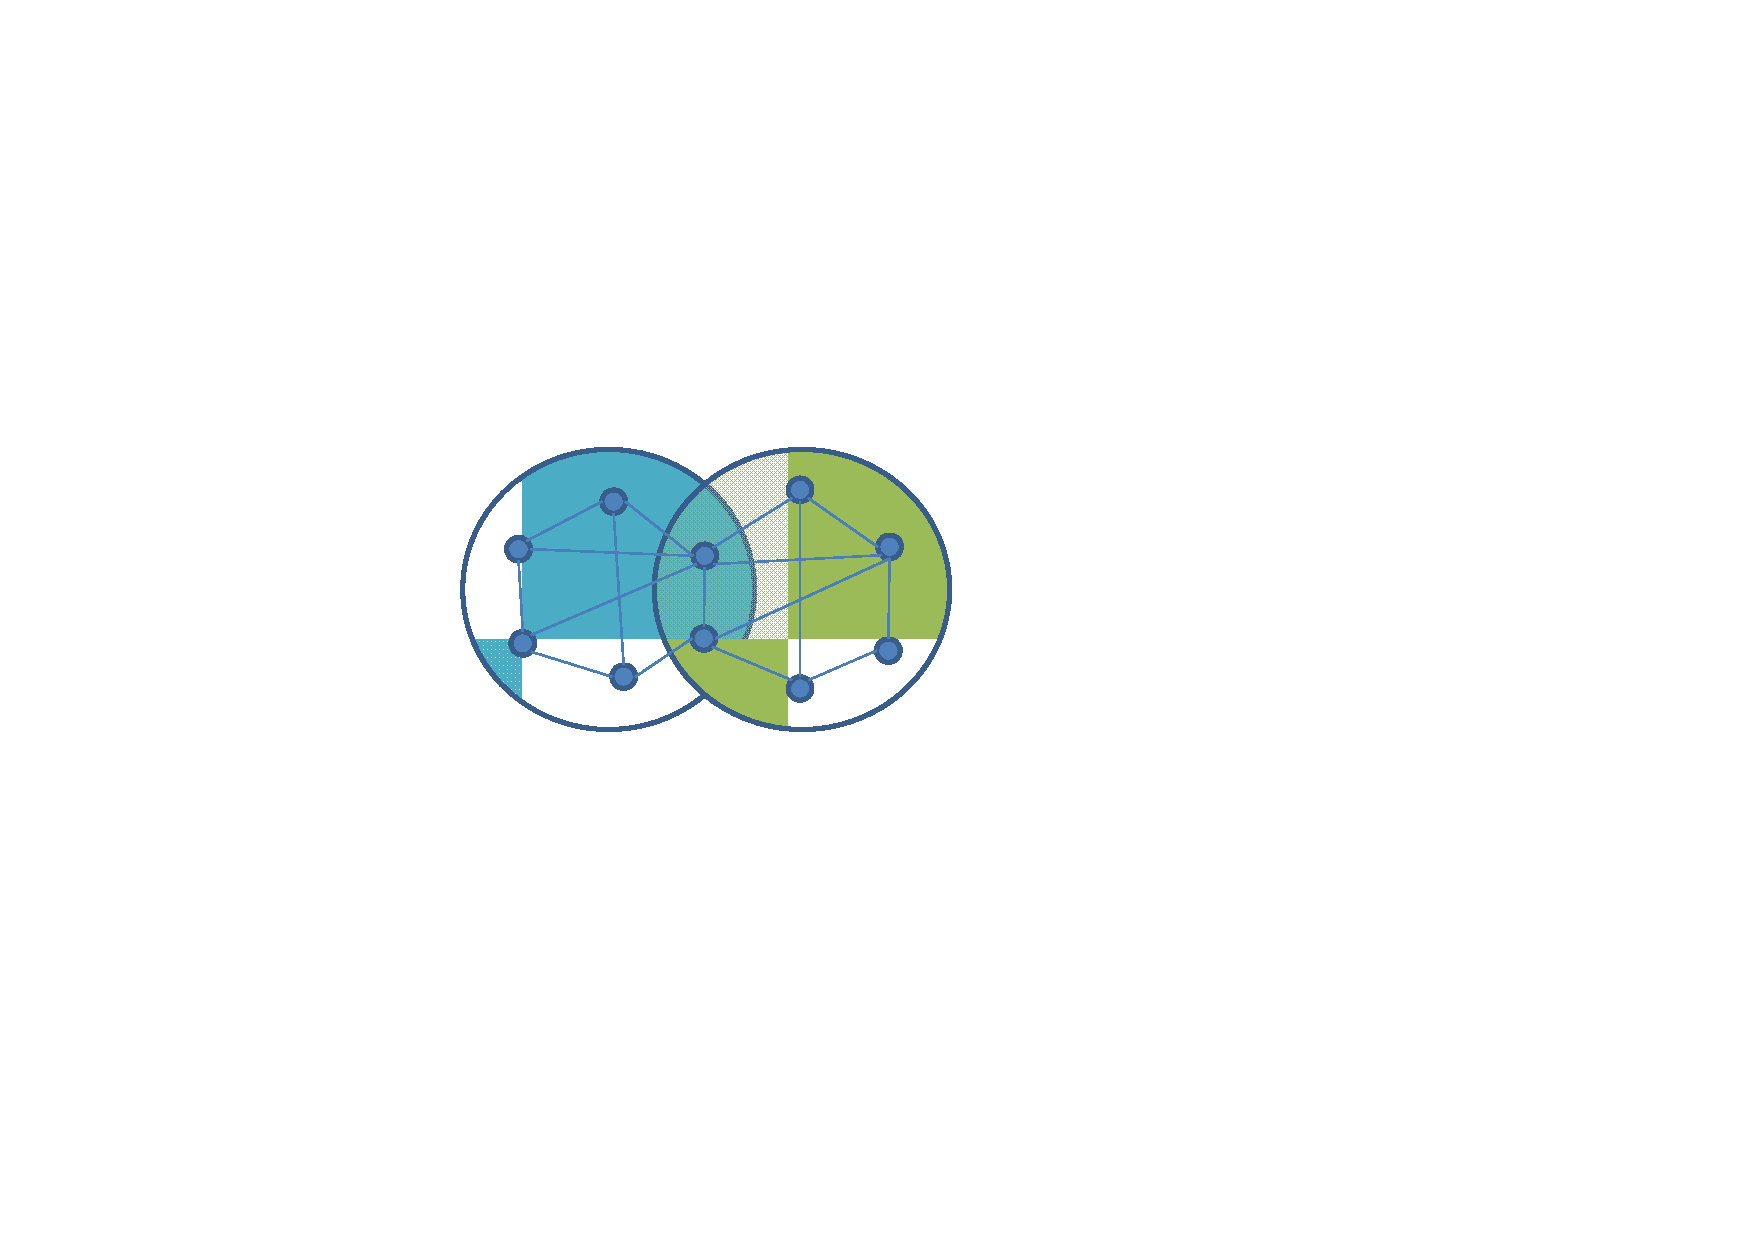
\includegraphics[height=0.14\textwidth]{figure/syn1.pdf}} &  \raisebox{-0.9\height}{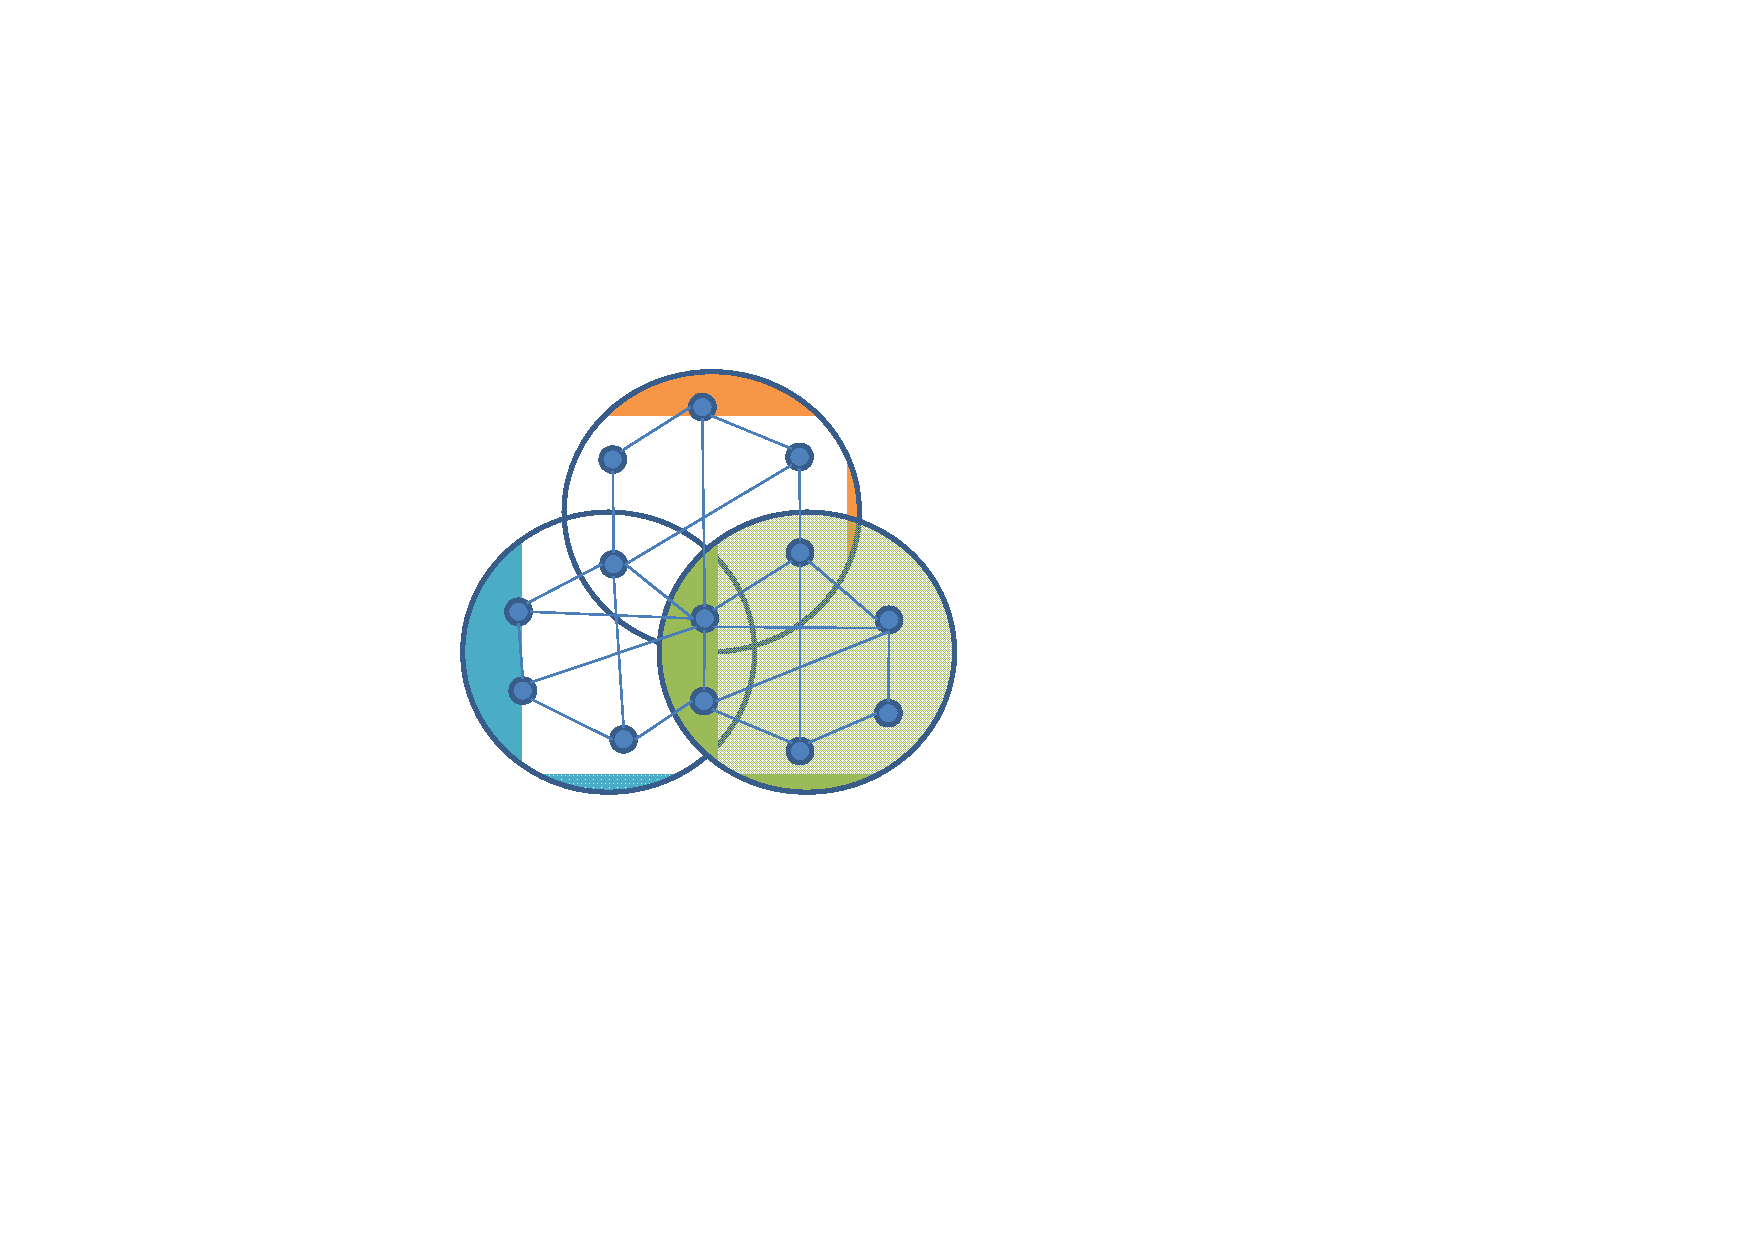
\includegraphics[height=0.14\textwidth]{figure/syn2.pdf}}  &  \raisebox{-0.9\height}{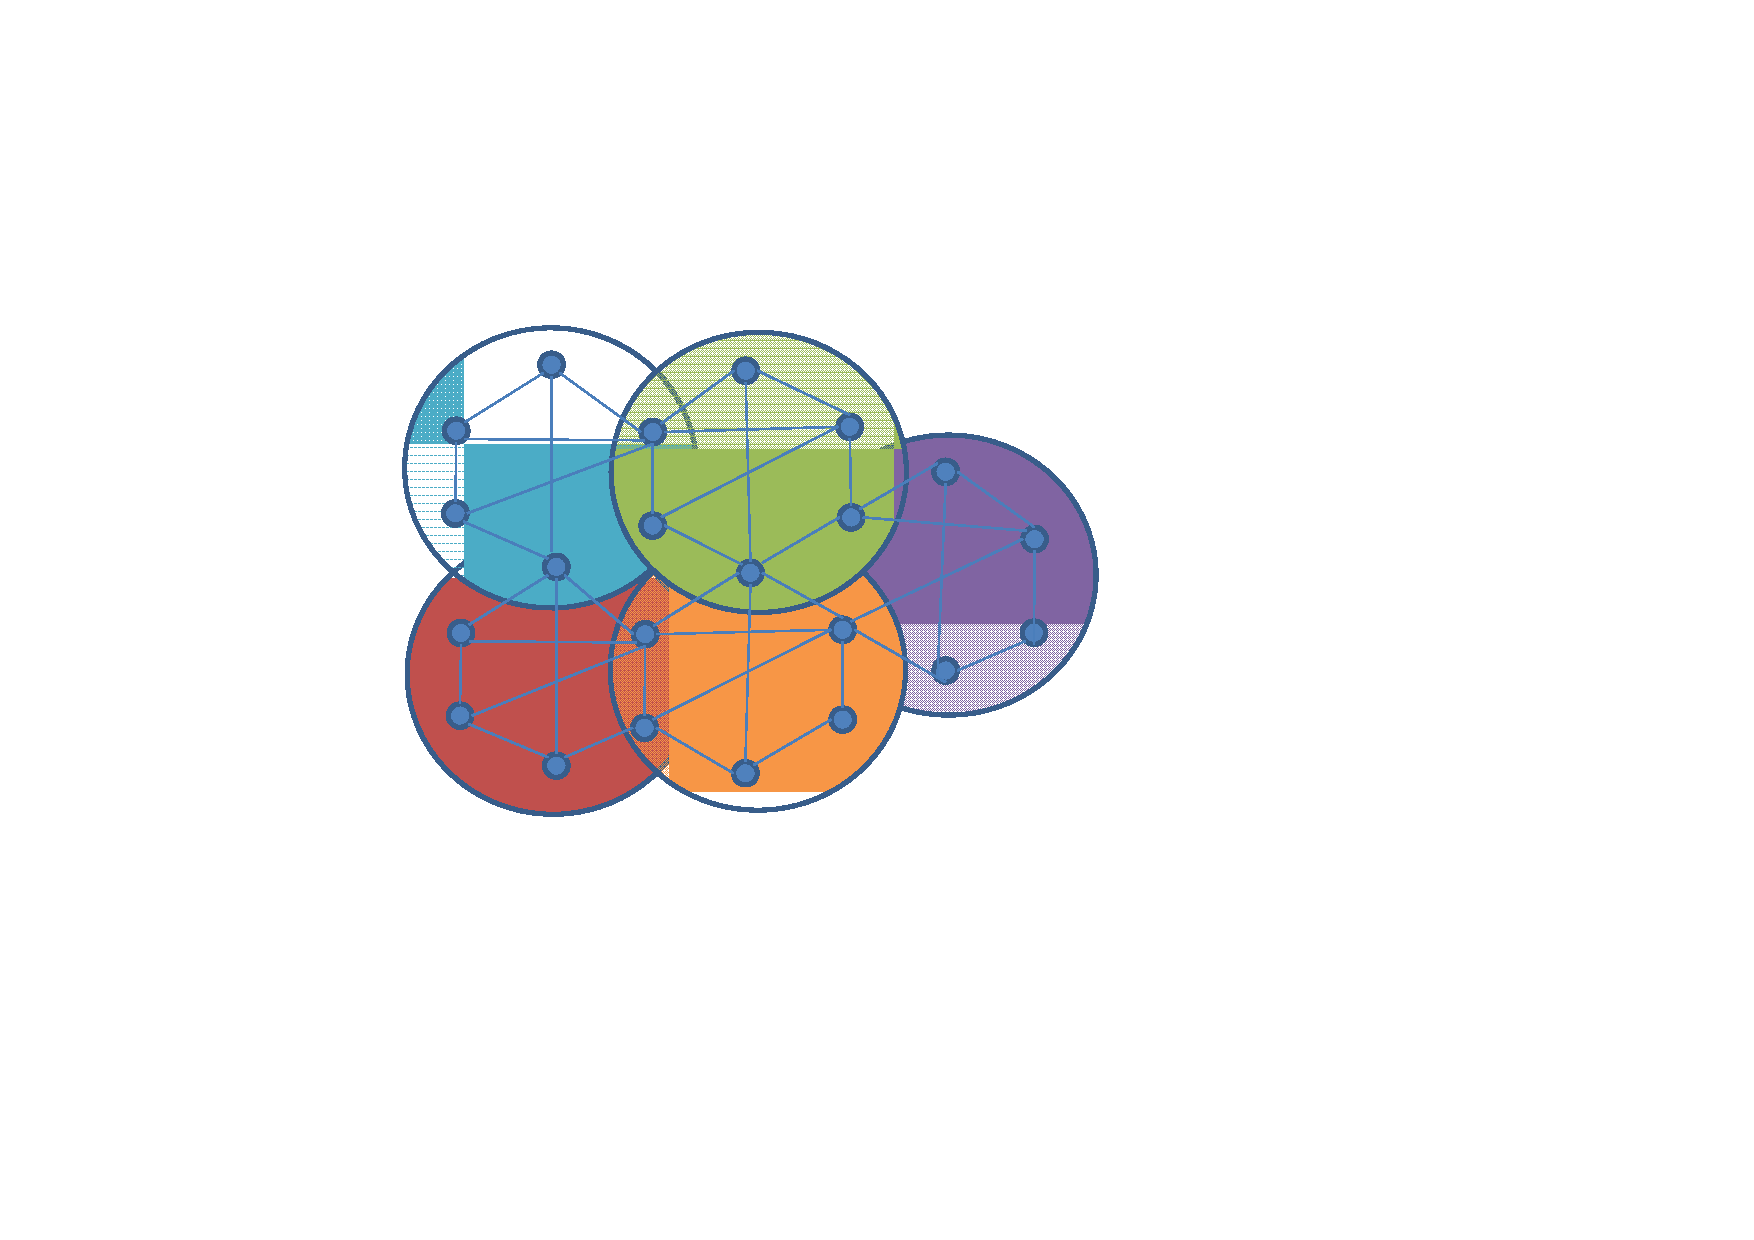
\includegraphics[height=0.14\textwidth]{figure/syn3.pdf}} \\
\hline 
Structure Setting &\tabincell{c}{$n_c = 200;n_o = 10;$\\$d_c = 0.8; d_b = 0.1$} & \tabincell{c}{$n_c = 200;n_o = 10;$\\$d_c = 0.8; d_b = 0.1$}&\tabincell{c}{$n_c = 200;n_o = 10;$\\$d_c = 0.8; d_b = 0.1$}\\
\hline
Attribute Setting&$n_d=5;n_{od}=2;r=0.05$&$n_d=8;n_{od}=2;r=0.05$&$n_d=10;n_{od}=2;r=0.05$\\
\hline
Subspace Setting& \tabincell{c}{$C1: \{1,2,...,5\}$\\$C2: \{3,4,...,8\}$ }&\tabincell{c}{$C1: \{1,2,...,8\}$\\$ C2: \{7,8,...,14\}$\\$C3: \{13,14,...,20\}$ } &\tabincell{c}{$C1: \{1,2,...,10\}$\\ $C2: \{9,10,...,18\}$\\$C3: \{17,18,...,26\}$ \\$C4: \{25,26,...,34\}$\\$C5: \{33,34,...,42\}$ }\\
\hline
%\multicolumn{4}{|c|}{\tabincell{c}{$n_c: No. vertices of each cluster; n_o: No. vertices of each overlapping; d_c: density of each cluster; d_b: density between clusters$}} \\
\end{tabular}
\label{tab:syn}
\end{table*}

%\begin{table}[t]
%\center\caption{Indexes of Generating Synthetic Attributed Graphs}
%\begin{tabular}{cc}
% \multicolumn{2}{c}{\raisebox{-0.9\height}{\includegraphics[width=0.45\textwidth]{figure/1.pdf}}} \\
% \raisebox{-0.9\height}{\includegraphics[height=0.25\textwidth]{figure/datasize.pdf}} &  \raisebox{-0.9\height}{\includegraphics[height=0.25\textwidth]{figure/dim.pdf}} \\
%\end{tabular}
%\label{tab:syn}
%\end{table}

\subsubsection{Evaluation of Clustering}
In this section, we evaluate IROC on three synthetic data sets and compare it to four relevant algorithms. PICS \cite{DBLP:conf/sdm/AkogluTMF12} is a compression based algorithm which clusters both vertices and binary attributes. BAGC \cite{DBLP:conf/sigmod/XuKWCC12} is a probability model based attributed graph partition method. DB-CSC \cite{DBLP:conf/pkdd/GunnemannBS11} is a density based algorithm which aims at detecting dense clusters with coherent subspace of attributes. It is designed for graph with numerical attributes,which chooses the attribute neighborhood if the distance of attributes of two vertices is smaller than a threshold $\epsilon$. The distance is defined as the maximum difference of all the attributes like $dist(x,y) = \max_{i\in\{1,...,T\} } |x[i]-y[i]|$. We integerize the categorical attributes of our synthetic data for DB-CSC and set $\epsilon < 1$, which means the attribute neighbors with exactly same category will be chosen. CONGO is an overlapping community detection method without considering node attributes which is adopted to compare the ability of detecting overlapping communities in structural part. Due to the multiple clustering assignments, we adopt F1-Measure to evaluate these algorithms on clustering vertices. F1-Measure is computed as the harmonic mean of Precision and Recall. Precision measures the accuracy of the detected clusters and Recall measures whether all clusters are detected.

\begin{table*}[t]
\center\caption{Evaluation Overlapping Clusters of Synthetic Data Sets}
\begin{tabular}{|c|c|c|c|c|c|c|c|c|c|}
\hline
\multirow{2}{*}{Algorithms}	& \multicolumn{3}{|c|}{Syn1} & \multicolumn{3}{|c|}{Syn2} & \multicolumn{3}{|c|}{Syn3} \\
\cline{2-10} 
      & Precision & Recall & F-Measure& Precision & Recall & F-Measure& Precision & Recall & F-Measure\\
\hline     
 IROC & \textbf{1} &\textbf{1} & \textbf{1}  & \textbf{1} & \textbf{0.973}& \textbf{0.986} & \textbf{1}& \textbf{0.963} & \textbf{0.981} \\
\hline
 PICS & 1 & 0.322 & 0.487 & 1 & 0.732& 0.846 & 0.563 & 0.670& 0.612\\
\hline
 DB-CSC &  0.895 & 0.826& 0.859 &$-$&$-$& $-$ & $-$&$-$ &$-$  \\
\hline
 BAGC &  1 & 0.947 & 0.973 & 0.955 & 0.607& 0.742 & 0.490 & 0.722& 0.584\\
\hline
 CONGO &  0.524 & 1 & 0.688 & 0.392 & 1& 0.563 &$-$&$-$ &$-$ \\
\hline 
\end{tabular}
\label{tab:fmeasuresyn}
\end{table*}

%\begin{table}[t]
%\center\caption{ The Output of Number of Clusters}
%\begin{tabular}{|c|c|c|c|c|c|c|c|}
%\hline
%Data sets & True & IROC  & PICS & DB-CSC & BAGC & DEMON\\
%\hline
%$Syn1$& 2 & 2 & 3  & 12 & 2 & 1 \\
%\hline
%$Syn2$& 3 & 3 & 3 & 23 & 3 & 6\\
%\hline
%$Syn3$& 5 & 5 & 10 & 26 & 5 & 12 \\
%\hline
%\end{tabular}
%\label{tab:clusnum}
%\end{table}

From Tab. \ref{tab:fmeasuresyn}, it is obvious that our proposed algorithm IROC outperforms the other algorithms. Generally, PICS and BAGC are not able to detect overlapping parts of graphs. DB-CSC outputs many small clusters with several overlapping vertices. However $6$ parameters have to be set. CONGO performs worse than IROC as well, which provides redundant results. Besides, it needs the number of clusters and the depth of local betweenness. Specifically, in $Syn1$ IROC achieves perfect $2$ clusters without any parameters, as shown in Fig. {\ref{fig:IROCsyn}}. From Fig. {\ref{fig:picssyn}}, parameter-free algorithm PICS outputs $8$ clusters, which splits two big cluster to several small ones. BAGC achieves $2$ clusters, which cannot detect overlapping part. DB-CSC outputs $19$ clusters and some clusters contain less than ten vertices. We run DB-CSC with $\epsilon=0.5$, $k_{min}=4$, $min_{pts}=5$,$r_{obj}=0.1$,$r_{dim}=0.1$ and $s_{min}=1$. For CONGO, we set the number of clusters to $2$ and the depth of local betweenness $h=2$. It detects a very large overlap between two clusters, which is far away from the truth. For $Syn2$, overlap exists among all the three clusters. The number of dimensions of each cluster is increased to $8$. IROC achieves $3$ perfect clusters. It also successfully detects the vertices which are assigned to all three clusters. PICS outputs $6$ clusters of vertices without overlapping. BAGC produces $3$ cluster. DB-CSC achieves no result after adjusting $6$ parameters several times and running the algorithm several days. The reason might be that DB-CSC is not applicable for dense graph with higher dimensional attributes. CONGO outputs $3$ clusters with very large overlapping parameterized with $h = 2$. $Syn3$ is more complex than the two synthetic data sets before. Similarly, IROC output $5$ good clusters. PICS partitions vertices to $7$ clusters. BAGC partitions vertices to $5$ clusters. DB-CSC still cannot output any results after increasing the number of dimension of each cluster to $10$. Due to the increased size of the data, CONGO can not achieve any results after several days running. 

\subsubsection{Evaluation of Subspace}
CONGO is designed for general graphs without node attributes and BAGC is not able to detect subspaces of attributes. PICS is an algorithm which aims at clustering the binary attributes and not at finding attributed subspaces of certain clusters. For example, Fig.\ref{fig:subspace} shows the attributed matrix of $Syn1$ after running IROC and PICS. Specifically, the size of the attributed matrix of IROC is $380 \times 8 $, where black points mean that the attribute is included in a subspace of a cluster. Two black blocks represent the clustering results of our IROC, which clearly shows the subspace of attributes and both overlaps on vertices and attributes. While the size of the attribute matrix of IROC is $380 \times 35 $. Black points mean that the vertices have corresponding categories and red lines demonstrate there are $5$ attributes clusters. It is difficult to judge which attributed clusters are part of subspace to represent the meaning of the cluster. In addition, subspaces of various clusters may contain overlap, while the clustering of attributes is not able to achieve overlaps. Besides, it is hard to obtain the binary image of DB-CSC due to the fact that too many clusters with subspace are produced. Therefore, we compare IROC with DB-CSC by evaluating F1-Measure of subspaces. Obviously, IROC achieves perfect results on every synthetic data set. The F1-Measure of DB-CSC on $Syn1$ is $0.13$, as there are many small clusters and the clustering results on structural part does not lead to detect accurate subspace. Besides, PICS obtain $10$ attributes clusters on $Syn2$ and $9$ attributes clusters on $Syn3$. Similarly, they provide no information of which attributed clusters are part of subspace to represent the meaning of the cluster.
 %
%\begin{figure}[h]
%\centering
%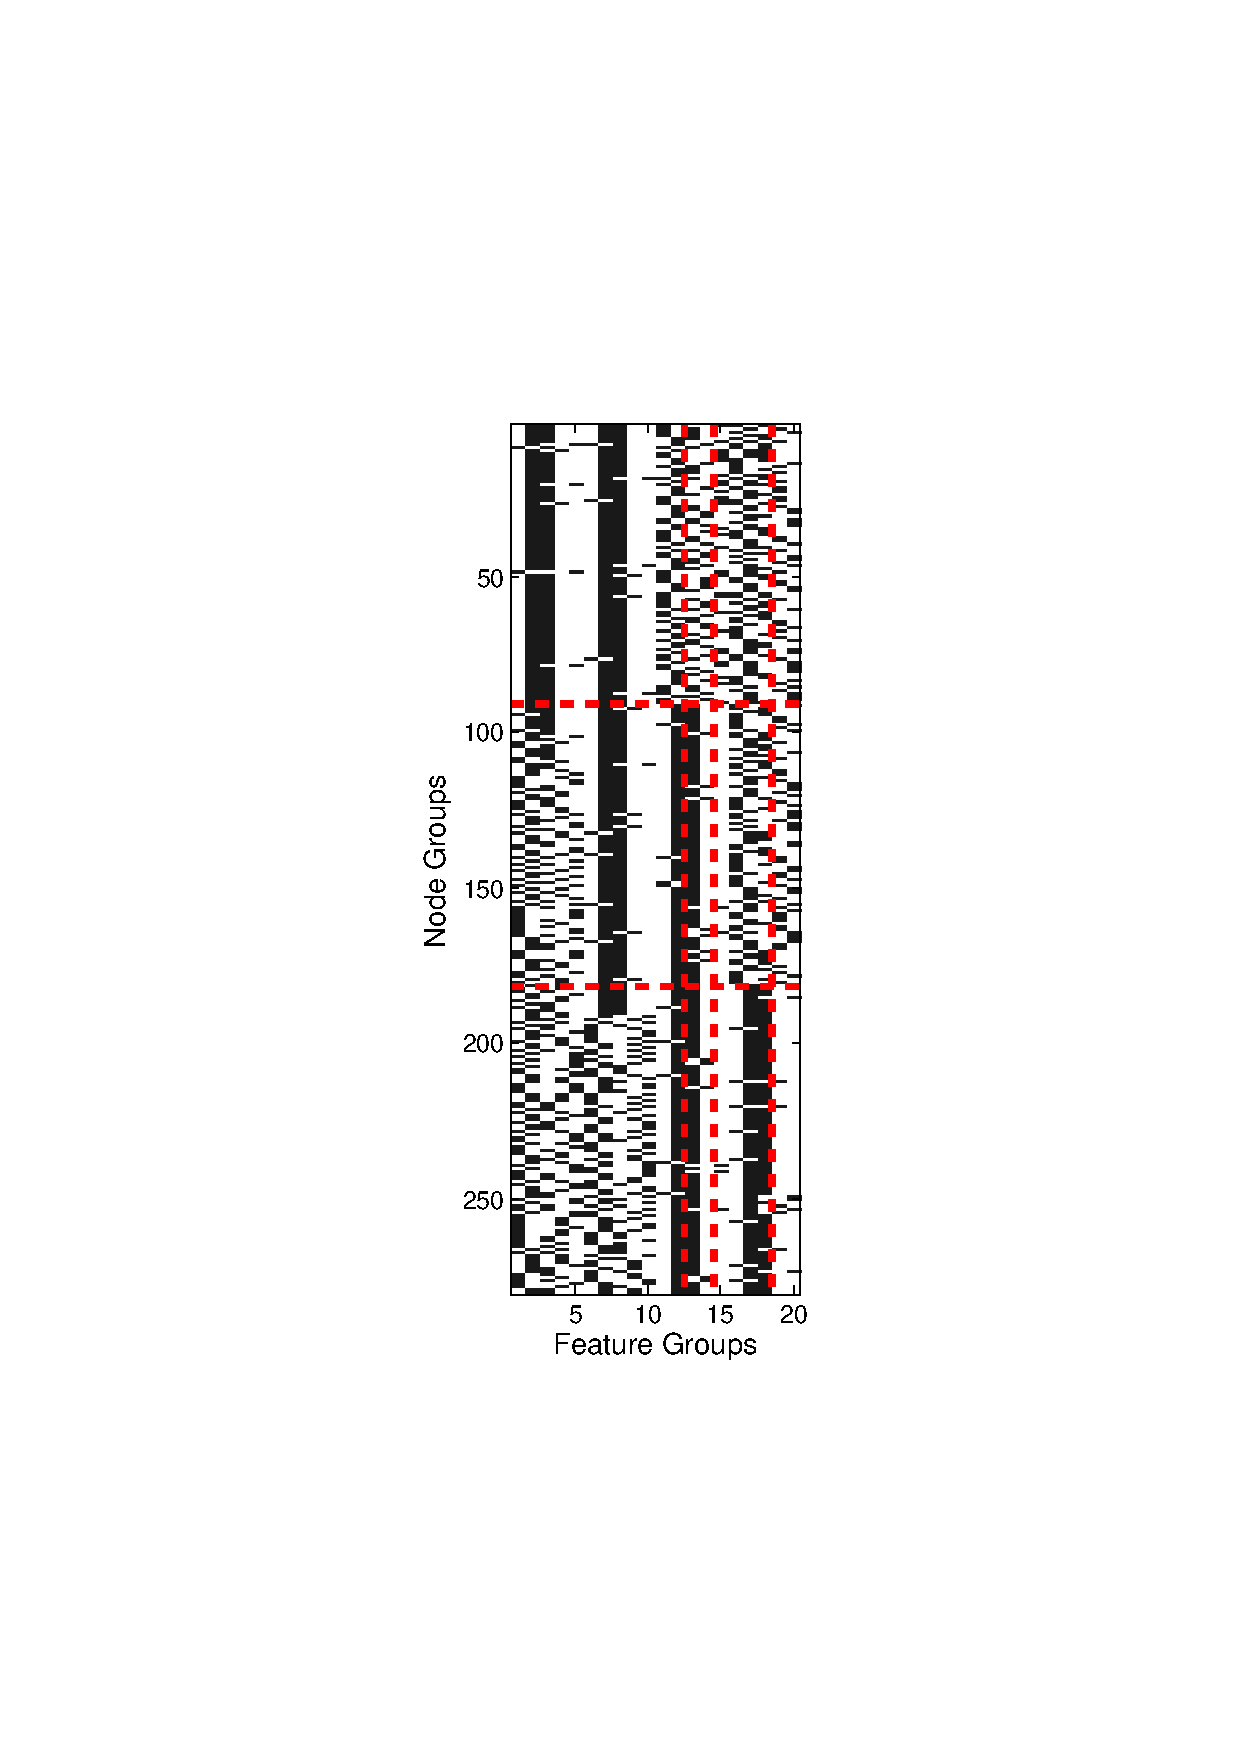
\includegraphics[height=0.8\columnwidth]{figure/3clusterPICS.pdf}
%\vspace{-3mm}
%\caption{Attribute Clustering of PICS on Syn2.}
%\label{fig:picssyn}
%\end{figure}

\begin{figure}	
	\centering
	\begin{subfigure}[h]{1.5in}
		\centering
		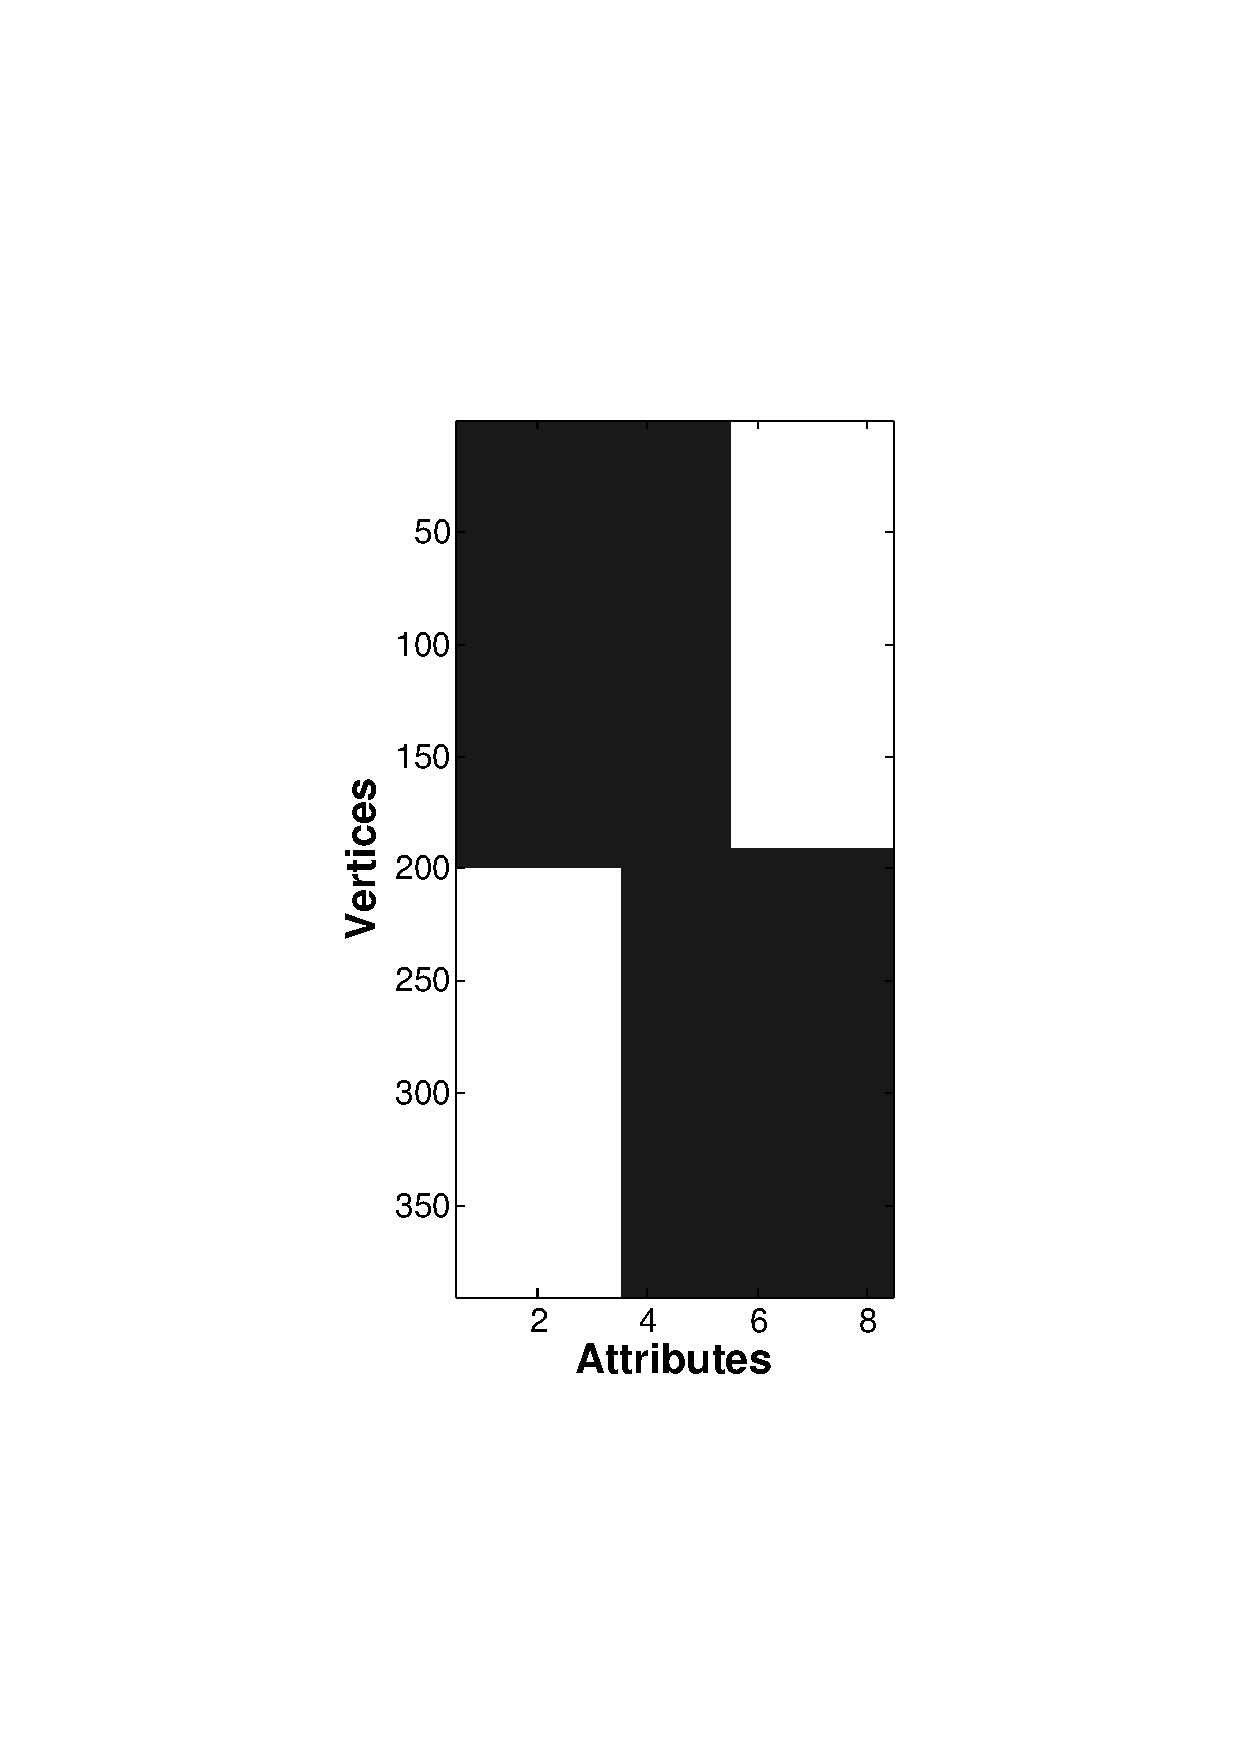
\includegraphics[height=2in]{figure/featurestander.pdf}
		\caption{IROC.}\label{fig:IROCsyn}		
	\end{subfigure}
	\quad
	\begin{subfigure}[h]{1.5in}
		\centering
		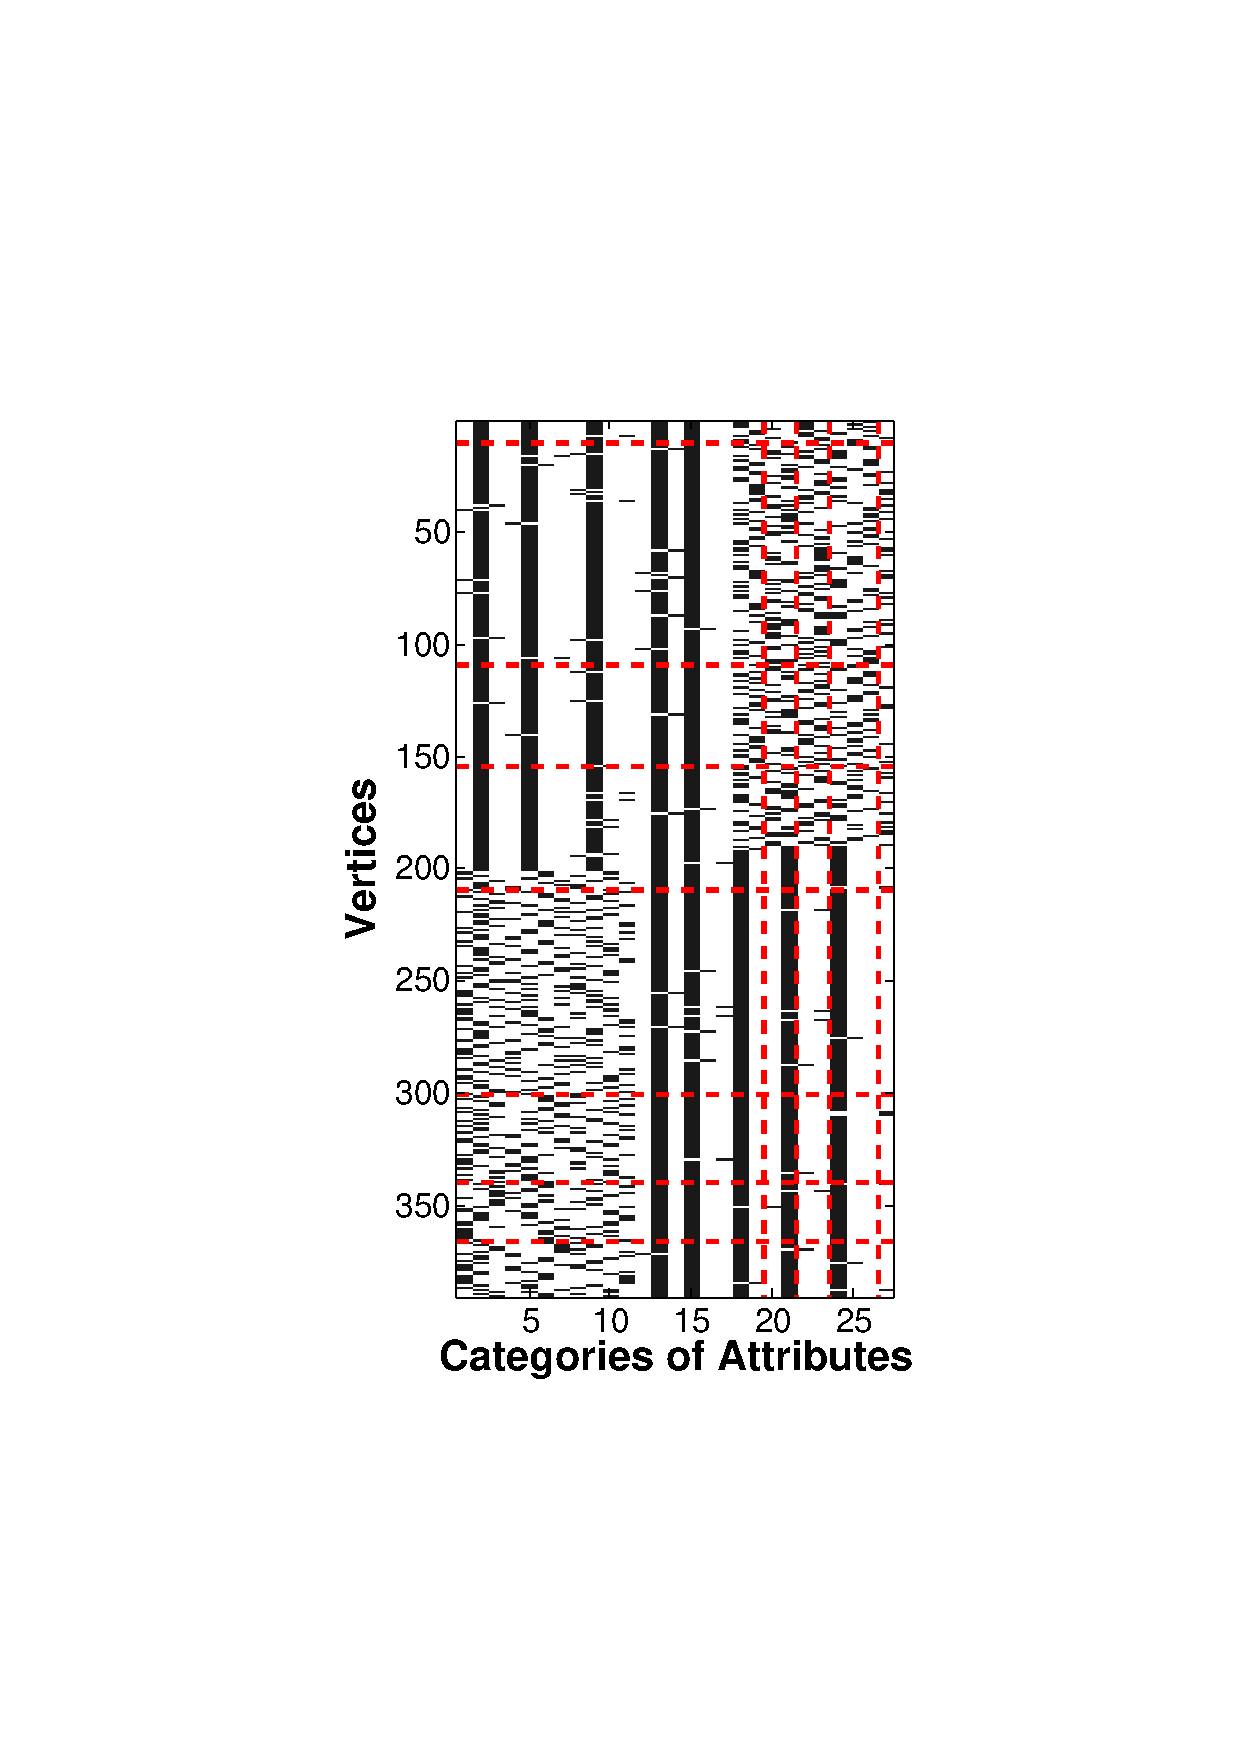
\includegraphics[height=2in]{figure/featurepics.pdf}
		\caption{PICS.}\label{fig:picssyn}
	\end{subfigure}
	\caption{Clustering Results of Syn1 in Attributed Matrix.}
	\label{fig:subspace}
\end{figure}


%\begin{table}[h]
%\center\caption{F1-Measure of Subspace}
%\begin{tabular}{|c|c|c|c|}
%\hline
%& Syn1 & Syn2 & Syn3 \\
%\hline
%$DocAG$& 1 & 1 & 1\\
%\hline
%$DB-CSC$& 0.333 & 0.155 & 0.090\\
%\hline
%\end{tabular}
%\label{tab:fmeasuresynsubspace}
%\end{table}
\subsection{Real Data sets}
\subsubsection{Facebook Data}
Facebook data sets are obtained from SNAP data sets \cite{DBLP:conf/nips/McAuleyL12}. Specifically, each Facebook data set is an ego-network of a selected node. For example, a network named $``1912"$ is generated by a node with id $1912$ and all its neighbors. Characters of vertices include birthday, education information, language, hometown, work information .etc. Each kind of property contains several anonymity items. The original node attributes are in binary form, and every single item is considered as an attribute. The value $``1"$ stands for the node that contains this item information and value $``0"$ vise verse. In this paper, we consider each type of property as attribute and the items in each property are defined as categories. In this section, we test two data sets: Ego-network $``1912"$ and Ego-network $``107"$. For the same reason with $Syn3$, we are not able to get the results from DB-CSC and CONGO after running the experiments for several days. Each data set is separated into several ``circles", but not all the vertices are included. That means only part of the vertices' label are available, thus we still use F1-Measure to compare the algorithms: IROC, PICS and BAGC. 

There are $755$ vertices in ego-network $``1912"$, and each vertex has $22$ attributes. Each attribute contains several categories, for example, there are $22$ categories in attribute "birthday" and $19$ categories in "education classes". The data set has already been labeled as $46$ circles. Obviously, Tab. \ref{tab:fmeasure1912} demonstrates that our proposed method achieves the best F1-Measure value by generating $12$ clusters. PICS generates $8$ clusters. The result of BAGC is acquired by setting the number of clusters to $46$, which equals to the given number of clusters. Ego-network $``107"$ contains $1045$ vertices, $23$ attributes and $9$ circles. Tab. \ref{tab:fmeasure1912} demonstrates that our proposed method IROC achieves the best F1-Measure value by generating $17$ clusters. PICS partitions vertices into $15$ clusters, and the result of BAGC is acquired by setting the number of clusters as $9$. Therefore, Tab.  \ref{tab:fmeasure1912} demonstrates that IROC has a big advantage in detecting vertex clusters.

\begin{table}[t]
\center\caption{F1-Measure of Facebook Data Sets }
\begin{tabular}{|c|c|c|c|c|c|}
\hline
Data sets & IROC  & PICS & BAGC \\
\hline
$Ego-network "1912"$& \textbf{0.231} & 0.224 & 0.229\\
\hline
$Ego-network "107"$& \textbf{0.141} & 0.101 & 0.118\\
\hline
\end{tabular}
\label{tab:fmeasure1912}
\end{table}

In addition, IROC discovers overlapping vertices between pairs of clusters. Take the Ego-network $``1912"$ data as an example, the analysis of overlapping is shown in Tab. \ref{tab:overlapping}. Specifically, Fig. \ref{fig:overlapping} shows a diagram of the overlapping part between cluster $C_2$ and cluster $C_{11}$. There are four overlapping vertices $``1941"$, $``2347"$, $``2468"$ and $``2543"$ forming a clique. Other vertices in $C_2$ and $C_{11}$ are both closely connected to the clique. Therefore, the two clusters $C_2$ and $C_{11}$ share the information of overlapping part and it is reasonable to assign overlapping vertices to both clusters.
\begin{table}[h]
\center\caption{Overlapping of Ego-network $"1912"$}
\small
\begin{tabular}{|c|l|}
\hline
Cluster ID & Overlapping Clusters ID(No.Vertices)\\
\hline
$C_1$ & $C_5$(1)\\
\hline
$C_2$ & \tabincell{c}{$C_3$(1), $C_4$(4), $C_5$(23), $C_6$(11), $C_7$(1), \\$C_8$(3), $C_9$(2), $C_{10}$(6) ,$C_{11}$(4), $C_{12}$(9)}\\
\hline
$C_3$ & $C_6$(1),$C_{11}$(15), $C_{12}$(4)\\
\hline
$C_4$ & $C_5$(1), $C_6$(1), $C_{11}$(11), $C_{12}$(12)\\
\hline
$C_5$ & $C_6$(1), $C_7$(1), $C_9$(1), $C_{12}$(3)\\
\hline
$C_6$ & $C_{10}$(1), $C_{12}$(3)\\
\hline
$C_{10}$ & $C_{11}$(1)\\
\hline
\end{tabular}
%\begin{tabular}{|c|c|}
%\hline
%Cluster ID & No.Overlapping \\
%\hline
%$C_1 \bigcap C_5$ & 1\\
%\hline
%$C_2 \bigcap C_3$ & 1\\
%\hline
%$C_2 \bigcap C_4$ & 4\\
%\hline
%$C_2 \bigcap C_5$ & 23\\
%\hline
%$C_2 \bigcap C_6$ & 11\\
%\hline
%$C_2 \bigcap C_7$ & 1 \\
%\hline
%$C_2 \bigcap C_8$ & 3\\
%\hline
%$C_2 \bigcap C_9$ & 2\\
%\hline
%$C_2 \bigcap C_{10}$ & 6\\
%\hline
%$C_2 \bigcap C_{11}$ & 4\\
%\hline
%$C_2 \bigcap C_{12}$ & 9\\
%\hline
%$C_3 \bigcap C_6$ & 1 \\
%\hline
%$C_3 \bigcap C_{11}$ & 15\\
%\hline
%$C_3 \bigcap C_{12}$ & 4\\
%\hline
%$C_4 \bigcap C_5$ & 1\\
%\hline
%$C_4 \bigcap C_6$ & 1\\
%\hline
%$C_4 \bigcap C_{11}$ & 1\\
%\hline
%$C_4 \bigcap C_{12}$ & 1\\
%\hline
%$C_5 \bigcap C_6$ & 1\\
%\hline
%$C_5 \bigcap C_7$ & 1\\
%\hline
%$C_5 \bigcap C_9$ & 1\\
%\hline
%$C_5 \bigcap C_{12}$ & 3\\
%\hline
%$C_6 \bigcap C_{10}$ & 1\\
%\hline
%$C_6 \bigcap C_{12}$ & 3\\
%\hline
%$C_{10} \bigcap C_{11}$ & 1\\
%\hline
%\end{tabular}
\label{tab:overlapping}
\end{table}

\begin{figure}[h]
\centering
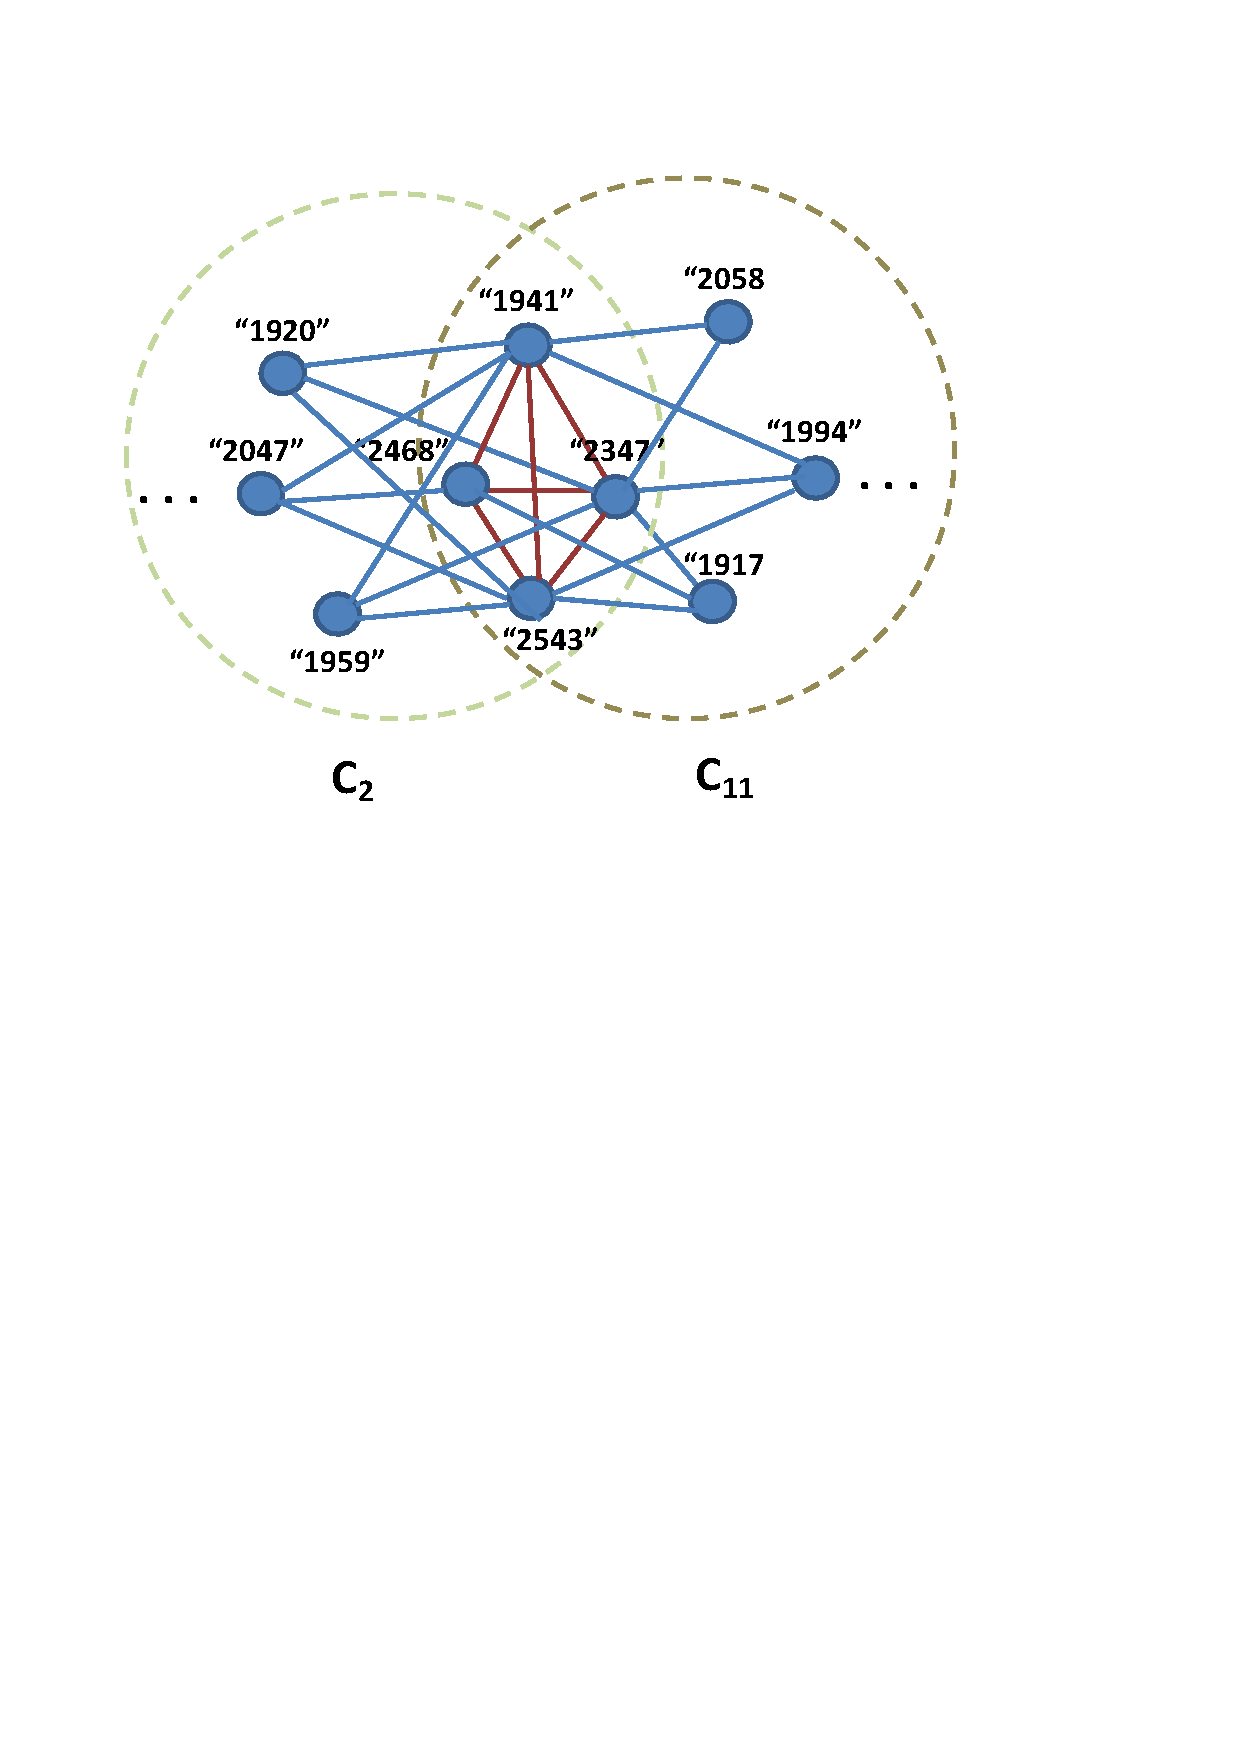
\includegraphics[width = 0.6\columnwidth]{figure/graph.pdf}
\vspace{-3mm}
\caption{Overlapping Between Cluster $2$ and Cluster $11$ of Ego-network "1912".}
\label{fig:overlapping}
\end{figure}

Betweenness centrality of a vertex is the ratio of the number of the shortest paths from $v_m$ to $v_n$ through vertex $v$ to the number of all shortest paths from $v_m$ to $v_n$ which is shown in Eq. (\ref{eq:betweenness}).
\begin{equation}
Betweeness(v)= \sum_{v_m\neq v\neq v_n}\frac{Path_{v_mv_n}(v)}{Path_{v_mv_n}}.
\label{eq:betweenness}
\end{equation}
Where betweenness centrality measures the ability of a human communicating with other humans in a social network \cite{betweeness}. That is to say, vertex with high betweenness plays the role of bridge. We calculate betweenness centrality of all the vertices, and rank them in descending order. Take the overlapping part of $C_2$ and $C_{11}$ as an example, the rank of the betweenness values of $``1941"$, $``2347"$, $``2468"$ and $``2543"$ is $5$, $4$, $20$ and $3$ separately, which possesses really high betweenness centrality values. Then these four persons are very outgoing and sociable. They communicate with various communities, so that they are assigned to multiple clusters. Besides, the betweenness values of all overlapping vertices are large, which implies that these vertices possess higher ability to communicate with other vertices thus assigning into multiple clusters.


%\begin{table}[h]
%\center\caption{Top 10 vertex Ranking by Betweeness Centrality}
%%\begin{tabular}{|c|c|c|c|c|c|c|c|c|c|}
%%\hline
%%Vertex ID & Rank & Vertex ID & Rank & Vertex ID & Rank & Vertex ID & Rank & Vertex ID & Rank &\\
%%\hline
%%"3497"& 24 & "3539" & 72 & "3632" & 5 & "3943" & 76 & "3504" & 143\\
%%\hline
%%"3761"& 20 & "3833" & 280 & "3971" & 91 & "3440" & 133 & "3522" & 4\\
%%\hline
%%"3559"& 131 & "3608" & 2 & "3666" & 148 & "3835" & 1 & "3896" & 101\\
%%\hline
%%"3934"& 271 & "3935" & 56 & "3590" & 79 & "3682" & 34 & "3507" & 75\\
%%\hline
%%"3561"& 174 & "3588" & 51 & "3597" & 93 & "3685" & 7 & "3763" & 82\\
%%\hline
%%"3798"& 42 & "3905" & 200 & "3911" & 71 & "3952" & 226 & "3556" & 94\\
%%\hline
%%"3710"& 6 & "3442" & 15 & "3633" & 87 & \\
%%\hline
%%\end{tabular}
%\begin{tabular}{|c|c|c|c|}
%\hline
%Rank & Vertex ID & Rank & Vertex ID \\
%\hline
%1 & \textbf{"3835"} & 6 & \textbf{"3710"}\\
%\hline
%2 & \textbf{"3608"} & 7 & \textbf{"3685"} \\
%\hline
%3 & "3923" & 8 & "3569"\\
%\hline
%4 & \textbf{"3522"} & 9 & "3621"\\
%\hline
%5 & \textbf{"3632"} & 10 & "3785" \\
%\hline
%\end{tabular}
%\label{tab:rank3437}
%\end{table}

Regarding the attributes, BAGC is not able to detect any subspace of clusters. PICS detects $8$ attributes clusters in Ego-network $``1912"$ and $11$ attributes clusters in Ego-network $``107"$. Our IROC detects a subspace of attributes for each cluster. Tab. \ref{tab:subspace1912} shows the attributes subspaces of Ego-network $``1912"$. The table shows that overlaps also exist between subspaces. For example, $C_5$ and $C_6$ have one vertex overlapping, and meanwhile their subspaces also overlap on attribute "middle name".

\begin{table}[h]
\center\caption{Subspace detected by IROC  of Ego-network $"1912"$}
\small
\begin{tabular}{|c|c|}
\hline
Cluster ID & Subspace\\
\hline
$C_1$ & all 22 attributes\\
\hline
$C_2$ & "middle name"\\
\hline
$C_3$ & "middle name","work projects"\\
\hline
$C_4$ & all 22 attributes\\
\hline
$C_5$ & "middle name","work projects"\\
\hline
$C_6$ & "middle name"\\
\hline
$C_7$ & all 22 attributes\\
\hline
$C_8$ & all 22 attributes\\
\hline
$C_9$ & all 22 attributes\\
\hline
$C_{10}$ & "work projects"\\
\hline
$C_{11}$ & "work projects"\\
\hline
$C_{12}$ & "middle name"\\
\hline
\end{tabular}
\label{tab:subspace1912}
\end{table}

%\begin{figure}[h]
%\centering
%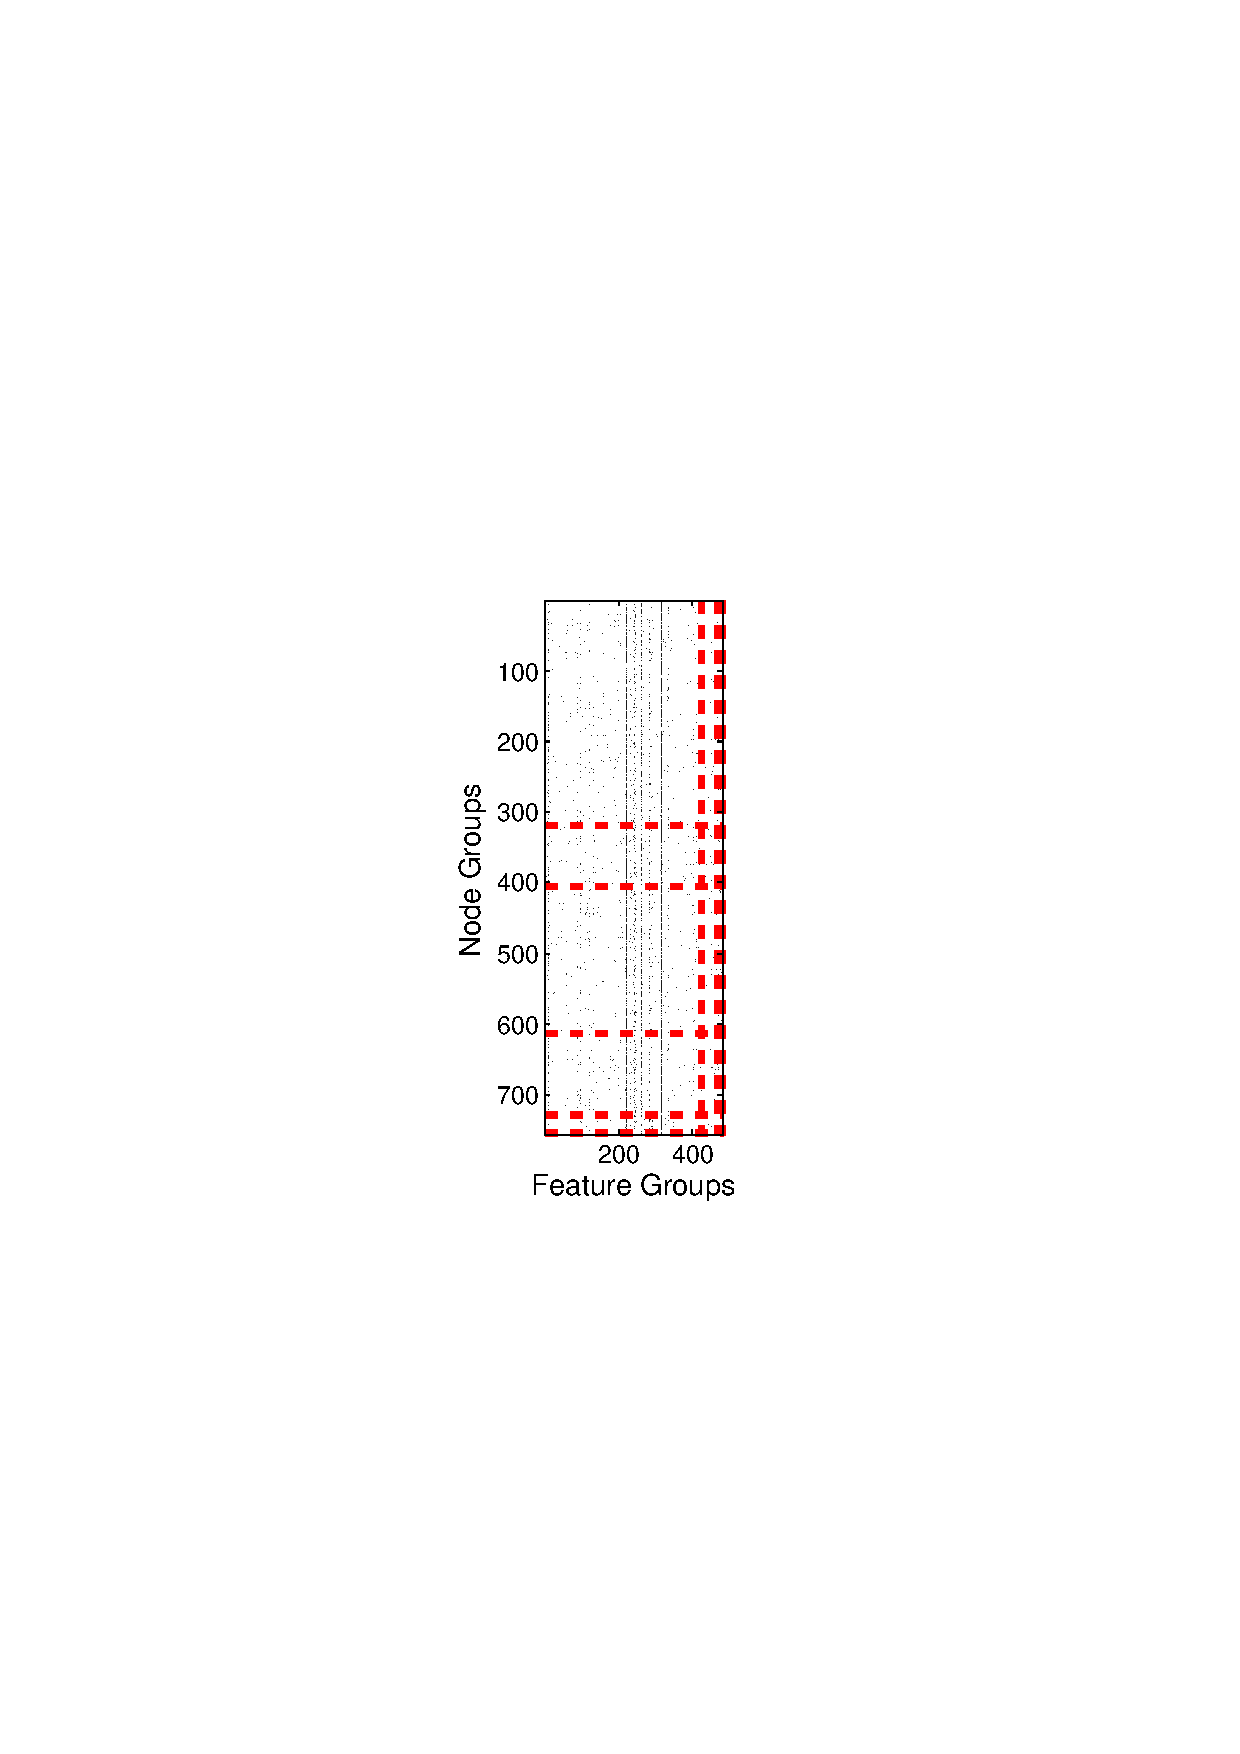
\includegraphics[height=0.5\columnwidth]{figure/PICS1912.pdf}
%\vspace{-3mm}
%\caption{Attribute Clustering of PICS on Ego-network "1912".}
%\label{fig:pics1912}
%\end{figure}


%\begin{table}[h]
%\center\caption{Subspace detected by IROC  of Ego-network $"107"$}
%\begin{tabular}{|c|c|}
%\hline
%Cluster ID & Subspace\\
%\hline
%$C_1$ & all 23 attributes\\
%\hline
%$C_2$ & all 23 attributes\\
%\hline
%$C_3$ & all 23 attributes\\
%\hline
%$C_4$ & "work with"\\
%\hline
%$C_5$ & all 23 attributes\\
%\hline
%$C_6$ & all 23 attributes\\
%\hline
%$C_7$ & all 23 attributes\\
%\hline
%$C_8$ & "middle name"\\
%\hline
%$C_9$ & all 23 attributes\\
%\hline
%$C_{10}$ & all 23 attributes\\
%\hline
%$C_{11}$ & "work from"\\
%\hline
%$C_{12}$ & "work projects"\\
%\hline
%$C_{13}$ & all 23 attributes\\
%\hline
%$C_{14}$ & "work projects"\\
%\hline
%$C_{15}$ & "education with"\\
%\hline
%$C_{16}$ & ""work from""\\
%\hline
%$C_{17}$ & all 23 attributes\\
%\hline
%\end{tabular}
%\label{tab:subspace107}
%\end{table} 
\newpage
\subsubsection{Google+ Data}
Google+ data sets are obtained from SNAP data sets \cite{DBLP:conf/nips/McAuleyL12} as well. Specifically, each Google+ data set is also an ego-network of a selected node. Similarly, we transfer the given binary feature to categorical feature which contains $6$ attributes: gender, institution, job title, last name, place and university. Similarly, part of labels are given as circles, thus we compare F1-Measure of the algorithms: IROC, PICS, BAGC and DBCSC. 

Tab. \ref{tab:fmeasuregp} shows that IROC achieves the best clustering result among all the algorithms. Take the data set $``gp53"$ which contains $1084$ vertices and $6$ attributes for example, our proposed algorithm IROC detects $17$ clusters with overlapping and without redundancy. Each cluster is provided with an attribute subspace which represents the meaning of the clusters. For example, people in one cluster are connected densely and all of them are from the same university, or people in one cluster are densely connected and all of them are from the same institution. Moreover, PICS outputs $12$ vertices clusters and $6$ attributes clusters. We set the number of cluster of BAGC to $4$, which equals to the given number of circles. DBCSC outputs $15$ clusters parametrized with $\epsilon=0.5$, $k_{min}=2$, $min_{pts}=3$,$r_{obj}=0.3$,$r_{dim}=0.3,s_{min}=3$. All the $15$ detected clusters are provided with a subspace. However, there are three clusters with exactly same vertices which contain redundant information.
\begin{table}[t]
\center\caption{F1-Measure of Google+ Data Sets }
\begin{tabular}{|c|c|c|c|c|c|}
\hline
Data sets & IROC  & PICS & BAGC & DBCSC \\
\hline
gp7 & \textbf{0.248} & 0.205 & 0.236 & 0.106\\
\hline
gp53 & \textbf{0.289} & 0.125 & 0.130& 0.074\\
\hline
\end{tabular}
\label{tab:fmeasuregp}
\end{table}